\chapter{Data}
\label{chp:data}

\section{Feature Design and Data Description}
\subsection{Raw Data - An AR}
\label{activeregion}
In this thesis, a single AR at some point in time (where $AR^i_t$ is the image of the $i'th$ AR at time $t$) is defined as a collection of a two dimensional continuum array ($C^i_t \in \mathbb{R}^{n\times m}$) and a magnetic field vector field of the same dimensions ($\vec{B} \in \mathbb{R}^{3 \times n\times m}$). These two images both constitute a single AR at a point in time (equation \ref{ardefinition}).
\begin{equation}
AR_t^i := \{C^i_t, \vec{B}\}
\label{ardefinition}
\end{equation}

The dimension $n\times m$ will be used to refer to a single AR dimension in terms of \textit{number of pixel rows} $\times$ \textit{number of pixel columns}; however, ARs vary in size.

The magnetic field was chosen in this project because areas of high magnetic flux essentially define ARs. I chose the continuum because it represents more visual aspects of the AR (which have been used extensively for flare forecasting).

One \textbf{AR} crossing the face of the solar disk is the object observed inside a \textit{Helioseismic Magnetic Imager AR Patch (HARP)} \cite{HARP} and is a subset of the solar surface that contains strong magnetic fields. The pipeline for extracting ARs is defined extensively in \cite{SHARP_Pipeline}. The Helioseismic and Magnetic Imager (HMI) continuously observes images of the sun and records roughly one terabyte of data every day, including a dopplergram, continuum, line of sight, and vector magnetograms. Although all three data products are helpful, I only use the continuum and magnetogram.

The \textbf{magnetogram} is a three dimensional vector field that measures the $x, y, z$ components of the sun's magnetic flux in Maxwells per $cm^2$ ($\frac{Mx}{cm^2}$). The $x, y$ components are the two components tangent to the solar surface, and the $z$ (often called the \textit{line of sight component}) is the magnetic field directed perpendicular to the surface of the sun. Therefore, the measure of magnetic flux must also measure the accumulation (average) flux for each pixel. In practice, JSOC separates the magnetogram into three separate two-dimensional arrays, each of size $n \times m$. Flares are more likely to occur in regions of higher magnetic flux.

The \textbf{continuum} is a two-dimensional array (of the same size as the magnetic field components - $n \times m$) that measures the continuum intensity of the solar surface. I chose to include the continuum because primary and reliable modern flare forecasting methods use an AR classification developed by McIntosh et al. \cite{MCintosh} where ``sunspots" (visually dark regions of the sun that are observable by the naked eye) are measured and compared to other sunspots. The local density, spacing, and size of sunspots are all used in the McIntosh scale as shown in figure \ref{fig:mcintoshclass}. 
%%%%%%%%%%%%%%%
\begin{figure}[h]
\centering
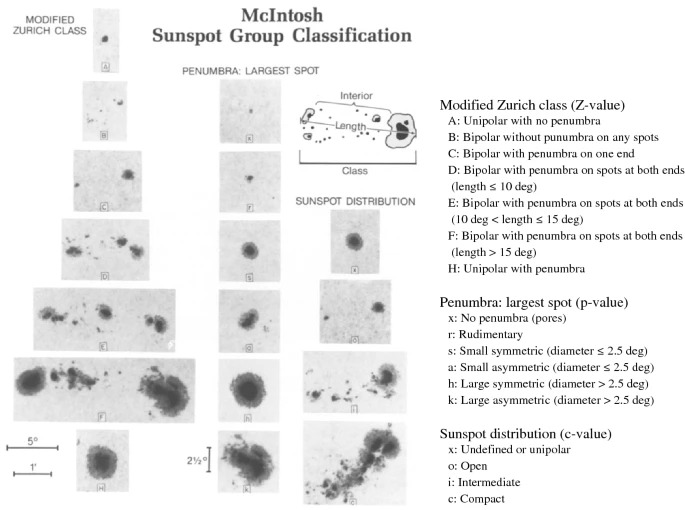
\includegraphics[width=0.5\linewidth]{ThesisFilePkg/figures/data/mcintosh.jpg}
\caption{McIntosh Classification System - measuring the continuum intensity of ARs shows distinct "sunspots" which are regions of \textit{low} intensity. Diagram from \cite{MCintosh}}
\label{fig:mcintoshclass}
\end{figure}
%%%%%%%%%%%%%%
The McIntosh classification system has been used extensively in flare forecasting methods, including Automated Solar Activity Prediction (ASAP, \cite{ASAP}). By including the continuum and magnetogram, I have access to a more general geometry and density measurement than the McIntosh classification system. \footnote{If done correctly, an algorithm that extracts umbrae and penumbrae is naturally going to be more general than a scientist labeling images}

\subsection{Feature Data - Segmentation}
\label{subregions}
Refer to appendix \ref{appendix:algorithms} for a detailed description of the algorithms for each Neutral Line, Umbra and Penumbra segmentation algorithm. This section will guide the reader through a high level description of the methods taken in order to segment the original AR. 

In order to turn a two-dimensional array into a meaningful mathematical ``object", I will be segmenting ARs based on widely used subsets, including the neutral line, umbra, and penumbra.

A Neutral Line is a continuous subset of an AR such that the line of sight magnetic field is $0$ and the gradient from positive to negative is relatively high. In this study, I use the fixed lower threshold of $150 \frac{Mx}{cm^2}$ (both positive and negative), a value chosen by Schrijver \cite{schrijver}).

Solar flares frequently occur in these polarity inversion regions with a high magnetic field gradient. It has been shown \cite{Properties2} that the length of the neutral line with horizontal shear greater than $80^o$ performed well in a one-variable discriminant analysis. This fact suggests that it is necessary to automatically detect the neutral lines or regions of high magnetic polarity and polarity inversion.

I find Neutral Lines computationally by first thresholding the image, then taking the dilation (an expansion/filling of holes) of positive flux and overlapping this dilation with negative flux to find the intersection of high gradient positive and high gradient negative regions. This step computes where a highly positive region drastically switches to a highly negative region. After finding areas of high gradient and zero magnetic flux, I will isolate ``clusters" of the neutral line, which are regions of densely packed zero flux, high gradient polarity inversion lines based on touching pixels - and group these clusters by labeling them by their total area multiplied by their total flux. This process is shown visually in figure \ref{fig:neutralline}.
%%%%%%%%%%%%%%%%%%%%
\begin{figure}[h]
\centering
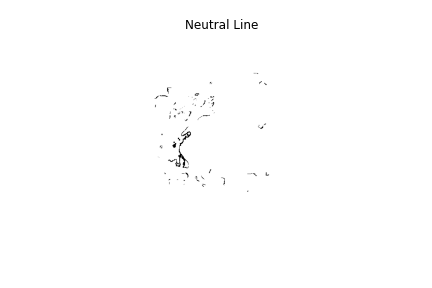
\includegraphics[width=0.5\linewidth]{ThesisFilePkg/figures/data/neutralline.png}
\caption{A neutral line shown visually. On the left is the original line of sight magnetogram; the middle shows the neutral line overlaid on top of the original magnetogram. The right image shows the isolated neutral lines (clustered based on whether pixels are touching).}
\label{fig:neutralline}
\end{figure}

When a high magnetic field exists in the photosphere, the surface traps heat in so-called ``flux tubes". The lower temperature surface ensures a lower intensity, which appears as a black or grey "sunspot" on the sun's surface. Often, an umbra will have an accompanying penumbra, or secondary low-intensity region, seen as a visually less dark region of the AR but still distinct from the rest of the surface. I will find Umbras and Penumbras using mathematical morphology using the first method described in \cite{comparisonofumpenmethod} (shown visually in figure \ref{fig:umbra} and \ref{fig:penumbra}).
%%%%%%%%%%%%%%%%%%%%
\begin{figure}[h]
\centering
\begin{subfigure}[b]{0.8\textwidth}
   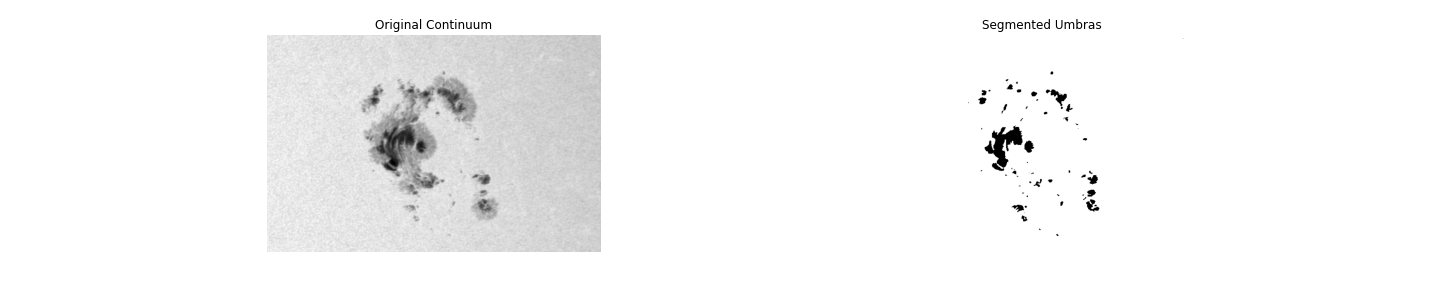
\includegraphics[width=\linewidth]{ThesisFilePkg/figures/data/umbras.png}
   \caption{}
   \label{fig:umbra} 
\end{subfigure}
\begin{subfigure}[b]{0.8\textwidth}
   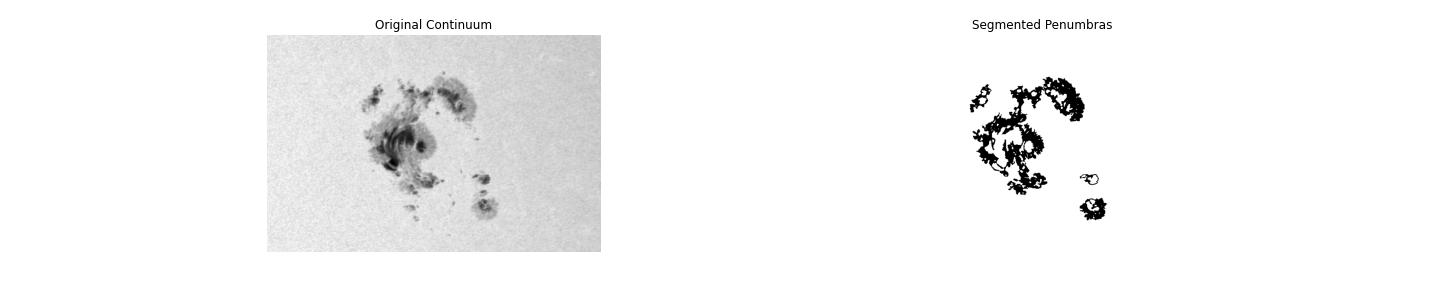
\includegraphics[width=\linewidth]{ThesisFilePkg/figures/data/penumbras.png}
   \caption{}
   \label{fig:penumbra}
\end{subfigure}
\caption[Umbra and Penumbra]{(a) An Umbra shown on an AR (shown on the left) and clustered (on the right) based on pixel intersections. (b) A penumbra showed on an AR and clustered.}
\end{figure}

The background is the complement of all other regions. The ``Background" is not a region used in solar flare forecasting. It is method-specific (that is, the shape of the background will be different depending on the method used to extract the neutral line and umbra/penumbra). 

I include the background to be comprehensive, so I am not ignoring the effects of what is happening just outside of each region. Indeed, when no other region is found (an AR has no neutral lines, umbras, or penumbras), some data should still be collected on this region. Also, I hypothesize that the effects of the magnetogram just outside of each region will affect the future shape and properties of each sub-region.

Note that the background is disjoint from all other subsets, the umbra is disjoint from the penumbra, but the neutral line is not necessarily disjoint from the umbra/penumbra.

\subsection{Feature Data - Parameterization}
Recent work (\cite{Properties1} \cite{Properties2} \cite{schrijver}) on characterizing flaring and non-flaring ARs have encouraged the use of scalar parameters based on the physical attributes of the AR. Although in any machine learning method, ``more data" is always encouraged, and the pruning of this data overtime to find the most optimal combination of variables speeds up and optimizes the entire forecasting pipeline, there are a few parameters that are continually associated with high flaring rates. In my preliminary work, I have chosen a set of 58 different scalars representing the physical, geometric or statistical properties of subregions of an AR. In this section, I will describe all 58 features, then describe the most important (based on prior work by Barnes et al. \cite{Properties1} \cite{Properties2} judging the relative impact of specific parameters towards flaring or non-flaring using a discriminant analysis).

For any of the multiple dimensional feature sets ($X$), I have chosen to summarize physical quantities using the first four standardized central moments: mean ($\mu$), standard deviation ($E(X - \mu)$), skewness ($E((X - \mu)^2)$), kurtosis ($E((X - \mu)^3)$). I will refer to these four moments as $M(X)$. Some of these formulas require scalar multiples of physical constants, but these will be left out because every quantity is normalized (discussed later in the methods section of this paper). All 58 features are defined in table \ref{fig:parameters}.
\renewcommand{\arraystretch}{1.8}
\begin{table}[p!]
\centering
\begin{tabular}{||c c c||} 
 \hline
 Property Description & Variable & Formula \\ [0.5ex] 
 \hline\hline
 Line of Sight Magnetic Field & $M(B_z)$ & $M(B_z)$\\ 
 \hline
 Total of Magnetic Flux Magnitude & $\Phi_{tot}$ & $\sum_{\Phi \in B_z}|\Phi|dA$ \\
 \hline
 Magnitude of Total Magnetic Flux & $|\Phi_{net}|$ & $|\sum_{\Phi \in B_z}\Phi dA|$ \\
 \hline
 Horizontal Magnetic Field & $M(B_h)$ & $B_h = |B_x| + |B_y|$ \\
 \hline 
 Inclination Angle & $M(\gamma)$ & $\gamma = arctan(\frac{B_z}{B_h})$ \\
 \hline
 $B$ Gradient & $M(\nabla B)$ & $B = |B_x| + |B_y| + |B_z|$ \\
 \hline
 $B_z$ Gradient & $M(\nabla B_z)$ & $M(\nabla B_z)$ \\
 \hline
 $B_h$ Gradient & $M(\nabla B_h)$ & $M(\nabla B_h)$ \\
 \hline
 Vertical Current & $M(J_z)$ & $J_z = \frac{\partial B_y}{\partial x} - \frac{\partial B_x}{\partial y}$ \\
 \hline
 Total of Vertical Current Magnitude & $I_{tot}$ & $I_{tot} = \sum_{j \in J_z}|j|dA$ \\
 \hline
 Magnitude of Total Vertical Current & $|I_{net}|$ & $|\sum_{j \in J_z}dA|$\\
 \hline
 Sum of Each Polarity Current & $|I_{net}^B|$ & $|\sum_{j \in J_z(B_z > 0)}jdA| + |\sum_{j \in J_z(B_z < 0)}j dA|$ \\
 \hline 
 Vertical Heterogeneity Current Density & $M(J_z^h)$ & $(\frac{1}{|B_x| + |B_y| + |B_z|})(B_y \frac{\partial B_x}{\partial y} - B_x \frac{\partial B_y}{\partial x})$\\
 \hline 
 Total of Vertical Heterogeneity Current Magnitude & $I_{tot}^h$ & $\sum_{i \in J_z^h}|idA|$ \\
 \hline
 Magnitude of Total Vertical Heterogeneity Current & $|I_{net}^h|$ & $|\sum_{i \in J_z^h}idA|$ \\
 \hline
 Twist & $M(T)$ & $T = \frac{J_z}{B_z}$ \\
 \hline
 Current Helicity & $M(h_c)$ & $h_c = B_z(\frac{\partial B_y}{\partial x} - \frac{\partial B_x}{\partial y})$ \\
 \hline
 Total of Current Helicity Magnitude & $h_{c tot}$ & $\sum_{h \in h_c}|h|dA$ \\
 \hline
 Magnitude of Total Current Helicity & $|h_{c net}|$ & $|\sum_{h \in h_c}h|dA$ \\
 \hline
 Shear & $M(\Psi)$ & $\Psi = arccos(\frac{\vec{B_p} \cdot \vec{B_o}}{B_oB_p})$ \\
 \hline
 Photospheric excess Magnetic Energy Density & $M(\rho_e)$ & $|B_p - B_o|$ \\
 \hline
 Total Photospheric Excess Magnetic Energy & $E_e$ & $\sum_{p \in p_e}dA$ \\
 \hline
 \end{tabular}
 \caption{A list of all 58 physical scalars currently used by my segmentation method extracted within a subset of an AR and used as inputs to the used machine learning algorithm}
 \label{fig:parameters}
\end{table}

\section{The Three Vector feature sets}
The type, structure, and organization of data in this project will be vital to extracting meaningful results. The intention of the feature extraction of the data collected from the HMI is to be as comprehensive as possible (as many physical features as possible). The three feature sets I will be extracting are theSFull, Segmented, and Graph feature sets. After obtaining a SHARP AR magnetogram and continuum from section \ref{activeregion} (the physical parameterization of this overall AR being the Full feature set), I will extract the three types of segments \textit{without clustering them} as described in section \ref{subregions} (the parameterization of these subsets of the AR is called the Segmented feature set). I will then cluster each subsection into ``nodes" and connect these nodes. This result will be called the graph feature set.

An AR ($AR_t^i$) is a collection of pixels, each with an x, y, z magnetic flux magnitude and a continuum scalar. Therefore, one can consider the AR as an element of $\mathbb{R}^{4 \times n\times m}$. Let $NL_t^i, UM_t^i, PU_t^i B_t^i\subset AR_t^i$ be subsets of the AR denoting the neutral line, umbra, penumbra and background, respectively. The function $P : \mathbb{R}^{4} \rightarrow \mathbb{R}^{58}$ takes in a subset of the solar surface and computes a vector of many physical features such as total magnetic flux, total shear, etc. 

The Full feature set is expressed in equation \ref{eq:Full}.
\begin{equation}
    D_{\text{Full}} = \{P(AR_t^i) \quad : \quad \forall AR_t^i\}
    \label{eq:Full}
\end{equation}
The Full feature set is simply the physical scalars of the entire AR. This feature set is a control.

The Segmented feature set is expressed in equation \ref{eq:Segmented}.
\begin{equation}
    D_{\text{Segmented}} = \{
    \begin{bmatrix}
    \restr{P}{NL_t^i}(AR_t^i) & , & \restr{P}{UM_t^i}(AR_t^i) & , & \restr{P}{PU_t^i}(AR_t^i) & , & \restr{P}{B_t^i}(AR_t^i)
    \end{bmatrix} \quad : \quad \forall AR_t^i \}
    \label{eq:Segmented}
\end{equation}
Where $\restr{A}{B}$ is the restriction of the function $A$ onto the subdomain $B$. The Segmented feature set represents each physical scalar vector for each segment. That is, it is a vector of four stacked vectors, each encoding physical features of their respective subset of the AR.

The graph feature set is not originally a vector like the other two. I wish to find static properties of individual subsets of the AR and the interaction of one subset with another. This notion of interaction brings to light the idea of a graph representation, where touching subregions are connected, and nodes on a graph represent individual regions. The graph feature set is slightly more complex than the previous two because it requires turning a \textbf{Segmented} AR into a graph, then turning this graph into a fixed-length vector.

Given a subset $S \subset AR_t^i$, node $j$ ($S_j$) is a subset of $S$ such that every pixel is touching (equation \ref{eq:touchingpixels}).
\begin{equation}
    S_j, S_k \subset S \qquad S_j \cap S_k = \emptyset \quad j \neq k
    \label{eq:touchingpixels}
\end{equation}
Two nodes $S_j$, $N_j$ (these can be the same or different types) are connected if their intersection of their dilation using a 3x3 kernel is non zero (equation \ref{eq:dilation}).
\begin{equation}
    dilation(S_j, square(3)) \cap dilation(N_j, square(3)) \neq \emptyset
    \label{eq:dilation}
\end{equation}
where the dilation of a region in morphology essentially ``expands and smooths" shapes the set by one pixel (equation \ref{eq:dilationdef}). I use a 3x3 kernel so that each centered active pixel expands one pixel in each direction (that is, a 3x3 kernel expands the set by 1 pixel, a 5x5 would expand it by 2 pixels, a 7x7 would expand it by 3 pixels, etc.):
\begin{equation}
    dilation(A, B) = \cup_{b\in B}A_b
    \label{eq:dilationdef}
\end{equation}
where $A_b$ is the translation of $A$ by $b$. This means that if regions are \textit{bordering} or \textit{intersecting}, they are connected. I chose the one-pixel grouping so that pixels can be a maximum of one pixel from one another. I could use a higher gap; however, this will be a controlled variable for the entirety of the experiment. The connection should measure ``bordering pixels," so the closer the pixels are, the better (and there is no smaller dilation than a 3x3 kernel). For each node, I collect the physical properties using a table of python functions that return physical quantities described above and tied to that node to create a homogeneous vertex embedded graph $G$.

\section{Statistical Analysis of the Three Feature Sets}
I designed the problem space to separate ARs into two classes: M+ flaring within 24 hours and M+ non-flaring within 24 hours. This thesis is primarily concerned with nonlinear relationships between variables and machine learning, but it is helpful to look at superficial statistical relationships to see any apparent trends in each feature set. An obvious example is that flaring regions tend to have a higher excess potential energy (often stored in their neutral line). Shown in figure \ref{fig:nlphi}, I observe the distribution of total excess potential energy within the Neutral Line for flaring and non-flaring ARs (left) and the total LOS Magnetic flux (right).
%%%%%%%%%%%%%%%%%%
\begin{figure}[h]
    \centering
    \includegraphics[width=\linewidth]{ThesisFilePkg/figures/data/feature setanalysis.png}
    \caption{KDE Distribution plot of 6601 M+ flaring in 24 hours and 6601 non-flaring ARs. The left plot promisingly shows that most non-flaring ARs had total neutral line potential energy near zero, and most flaring ARs had higher neutral line potential energy. Note that this distribution plot balances the number of flaring and non-flaring data points.}
    \label{fig:nlphi}
\end{figure}
These plots are generated by balancing the number of flaring and non-flaring ARs, then creating two histograms. I balanced flaring and non-flaring in this case only to show the difference between the two classes, and the rest of this paper assumes a more realistic ratio of flaring to non-flaring ARs. The flaring data (light blue) is essentially an inverted density histogram, where each "bin," or x-axis label sums the percent of ARs that fall in that bin that flare and do not flare to 1. Note that the data comes from a balanced feature set. So there are 6601 M+ flaring ARs and 6601 non-flaring ARs in total in the entire plot. So the seemingly dominating upper end of the neutral line potential energy plot shows that given the neutral line potential energy is immense, the probability of flaring is significant. That is, $p(Flaring \quad | \quad \rho >> 0) \quad > \quad p(Flaring \quad | \quad \rho \quad near \quad 0)$, and a similar statement is made for the distribution of total LOS penumbra flux, but to a lesser degree.

Figure \ref{fig:nlphi} does not necessarily offer a threshold or method to separate flaring/non-flaring regions because I observe that some non-flaring regions have a high potential energy of their neutral lines. However, it separates flaring and non-flaring regions in their excess potential energy. In general, the probability that an AR is flaring is higher if it has a higher neutral line excess potential energy for the total flux of the penumbra. This analysis, however, is an observational one, and my feature analysis chapter goes into a more in-depth review of the ranking of features across \textit{all three feature sets}.

\section{Feature Set Limitations} \label{sec:limitations}
\textit{Parameter tuning of the neutral line makes a difference}. In the algorithm to extract the Neutral Line, I use a lower threshold value of $150 \frac{Mx}{cm^2}$ before the positive and negative subsets are dilated and compared. This threshold is an arbitrary number, and some ARs require a higher or lower threshold value. A possible solution to this issue would be to adaptively estimate a threshold value based on the total magnetic flux. For example, use the $60\%$ standard deviation of the total magnetic flux as the lower end threshold. However, this would ignore that some ARs with more neutral lines do not have a higher probability of flaring than an AR with a single, high flux gradient neutral line. I chose a static flux gradient threshold to remain consistent, so the measurement of the geometry and size of the neutral line is maintained. 

\textit{Parameter tuning of the umbra and penumbra makes a difference}. The threshold value of 21000 is chosen arbitrarily from experimentation but removes the accuracy of a human-labeled umbra and penumbra. Typically, umbras and penumbras seem apparent to the observer but are more challenging to segment using an algorithm. Previous methods of umbra penumbra segmentation used set-level image segmentation and simple statistical segmentation, but none seemed to work as well as the currently proposed segmentation method using localized adaptive threshold and basic image morphology. A possible solution could include adding a pipeline that extracts umbras and penumbras using computer vision and convolutional neural networks, but this is out of the scope of this library. The library, as it stands, is designed modularly, and changing the algorithm for each segmentation does not ruin the rest of the methods, so I can still do future work to tune the algorithm as it is now.

\textit{There is no global record of umbras, penumbra, and neutral lines through time}. This feature set works well for static images for each AR but is poorly designed for time series data. If a flare forecasting method attempts to record the physical parameterization over time by leaving out subsets of each AR based on size, some subsets are ignored and appear/disappear over time. For example, a single Umbra that traverses the length of the AR could be miss identified or ignored as we take a look at later images of the same AR.